\documentclass[%margin%,line,pifont,palatino,courier
]{article}
\usepackage{fullpage}
\usepackage{lastpage}
\usepackage[top=1in,bottom=1in,margin=1in]{geometry}
\usepackage{supertabular}
\usepackage{graphicx,tikz}	
%\usepackage{tkz-euclide}
%\usetkzobj{all}
%\usetikzlibrary{calc}
\usepackage{array,multicol}
\usepackage{amsmath,amssymb}
\usepackage{enumitem}

\usepackage{fancyhdr}
\pagestyle{fancy}

\addtolength{\topmargin}{-0.25in}

\newcommand{\vect}[1]{\mathbf{#1}}
\DeclareMathOperator{\proj}{proj}

\fancypagestyle{plain}{
	\addtolength{\headheight}{0.485in}
	\rhead{\bf MATH 236 (Calculus II) \\
		%\vspace{0.5pc}
		due Mon 18 Sep 2017 \\}
	\rfoot{\footnotesize THQuiz 2, p. \thepage\ (of \pageref{LastPage})
	}
\renewcommand{\headrulewidth}{0pt}
}
\fancyhf{}
\renewcommand{\headrulewidth}{0pt}
\rfoot{\footnotesize THQuiz 2, p. \thepage\ (of \pageref{LastPage})$\;$}

\title{\vspace{-3.5pc} 
	\flushleft \bf \Large Take-Home Quiz 2:  Integration techniques  %\\ 
	 (\S5.3-5.5)}
\date{}

% % % % %
\begin{document}
\maketitle

\vspace{-3pc}
\noindent{\bf Directions:} This quiz is due on September 18, 2017 at the beginning of lecture.  You may use whatever resources you like -- e.g., other textbooks, websites, collaboration with classmates -- to complete it \textbf{but YOU MUST DOCUMENT YOUR SOURCES}.  Acceptable documentation is enough information for me to find the source myself.  Rote copying another's work is unacceptable, regardless of whether you document it.  

\noindent\hrulefill

\begin{enumerate}
% % %
\item \begin{enumerate}
	\item {\bf \S5.3 \#12} Try to perform a partial-fraction decomposition of the improper rational function $\displaystyle\frac{x^3}{(x-1)(x-2)}$, without using long division.  What goes wrong?
	\item {\bf \S5.3 \#14} What goes wrong if you try to decompose $\displaystyle\frac{1}{(x^2+1)^2}$ into the form $\displaystyle\frac{A}{x^2+1}+\frac{B}{(x^2+1)^2}$?
	\end{enumerate}

% % %
\item Compute the integrals.
	\begin{enumerate}
	\item {\bf \S5.3 \#54} $\displaystyle\int\frac{e^x}{e^{3x}-2e^{2x}}\ dx$
	\item {\bf \S5.3 \#56} $\displaystyle\int\frac{\ln x+1}{x\left((\ln x)^2-4\right)}\ dx$
	\end{enumerate}
	
% % %
\item Describe strategies for solving the following types of integrals (see the table on p. 445).
	\begin{enumerate}
	\item {\bf \S5.4 \#10} $\int\cot^kx\ dx$, $k$ odd
	\item {\bf \S5.4 \#12} $\int\csc^kx\ dx$, $k=2$
	\item {\bf \S5.4 \#14} $\int\sin^mx\cos^nx\ dx$, one of $m$ and $n$ odd
	\item {\bf \S5.4 \#16} $\int\sec^mx\tan^nx\ dx$, $m$ even
	\item {\bf \S5.4 \#18} $\int\sec^mx\tan^nx\ dx$, $m$ odd and $n$ even
	\end{enumerate}

% % %
\item {\bf \S5.5 \#92}  The main cable on a certain suspension bridge follows a parabolic curve with equation $f(x)=(0.025x)^2$, measured in feet:  
\begin{center}
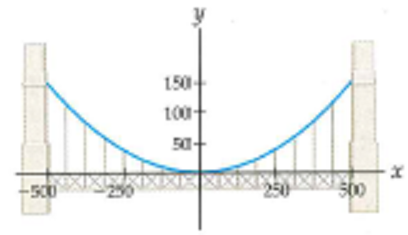
\includegraphics[scale=0.75]{5-5_92TaalmanKohn}
\end{center}	
	\begin{enumerate}
	\item  In general, the length of a curve $f(x)$ from $x=a$ to $x=b$ can be calculated from the formula
	\[
	\int_b^a\sqrt{1+(f'(x))^2}\ dx.
	\]
	Write down a specific definite integral that represents the length of the main cable of the suspension bridge.
	\item Use trigonometric substitution to solve the definite integral and determine the length of the cable.
	\end{enumerate}

% % %
\item {\bf \S5.5 \#94} Using part (a) as a guide, prove part (b) of Theorem 5.18:
\begin{quote}
For $x\in (-\infty, \infty)$ and $u\in (-\frac{\pi}{2},\frac{\pi}{2})$, the substitution $x=a\tan u$ gives $x^2+a^2=a\sec u$. 
\end{quote}
Your proof should include a discussion of domains and a consideration of absolute values.

% % % % %
\end{enumerate}
\end{document}